\section{Robótica}
\label{sec:robotica}

La palabra Robot se deriva de la palabra de origen checoslovaco robota, que quiere decir siervo. Dicha palabra apareció por primera vez en la literatura en la obra R.U.R (1921)(Robot Universalis de Rossum), de Karel Capek.

Un robot es un sistema electromecánico que utiliza una serie de elementos hardware
(actuadores, sensores y procesadores) y cuyo comportamiento viene controlado por un
software programable que le da la inteligencia. La robótica se puede ver como la ciencia
y la tecnología de los robots, donde se combinan varias disciplinas como la mecánica, la
informática, la electrónica y la ingeniería artificial, que hacen posible el diseño hardware y software del robot.

Los robots se componen esencialmente de tres tipos de dispositivos: sensores,
procesadores y actuadores. En un robot los sensores son los encargados de recoger
la información del entorno. En este grupo se situarían: el láser, el sonar o las
cámaras. Estos dispositivos equivaldrían a nuestros sentidos humanos. Por otro lado se
encuentran los procesadores, encargados de analizar los datos que le son suministrados
por los sensores, también son los encargados de elaborar una respuesta a estos datos y
enviar la acción que deba llevarse a cabo a los actuadores, son como nuestro cerebro.
Por último los actuadores, principalmente motores eléctricos, se encargan de interactuar
con el entorno del mismo modo que lo hacen nuestros músculos.


\subsection{Historia}
\label{subsec:historia}
A finales del siglo XIX se presentan las primeras máquinas \textit{robots}, pero no
será hasta la segunda guerra mundial cuando se realicen los primeros diseños de esta
naturaleza.Con el desarrollo de las primeras computadoras digitales se produjo una
considerable evolución en este campo. Así, en 1970 una serie de investigadores del
Instituto de Investigación de Stanford desarrollaron Shakey (figura 1.1). Su sistema de
control creaba una reproducción interna del entorno a partir de los sensores de que
disponía y desde ella calculaba su movimiento.

Aunque es un termino relativamente nuevo y cuyo uso extendido es muy reciente, la historia lleva siglos dando pasos para llegar al punto en el que nos encontramos.
Durante la época de los griegos se intentó crear dispositivos que tuvieran un movimiento sin fin, que no fuera controlado ni supervisado por personas, en los siglos XVII y XVIII la construcción de autómatas humanoides fabricados con mecanismos de relojería por Jacques de Vaucanson, Pierre Henri-Louis, Jaquet- Droz, como el escribiente, the Draughtsman, el músico Henri Maillar det (1800), Olimpia de la ópera de Offenback de Hoffman, fortalecieron la búsqueda de mecanismos que auxiliaran a los hombres en sus tareas.

Es En 1926  con \textit{Metrópolis} , de Fritz Lang, la primera película en la que aparecen robots cuando se empieza a dar a conocer el termino de forma popular.
En 1950 Isaac Asimov publica el libro \textit{Yo Robot}, con las tres leyes de la robótica:
\begin{itemize}
\item \textit{Un robot no puede lastimar a un ser humano o permanecer inactivo ante un daño que se le pueda hacer.}

\item \textit{El robot debe obedecer al ser humano excepto si contradice la primera ley.}

\item \textit{El robot debe proteger su existencia salvo que entre en conflicto con las leyes anteriores.}

\end{itemize}

Gracias a este libro, Isaac Asimov hizo popular la robótica.
Durante la Segunda Guerra Mundial aparecieron gran variedad de
mecanismos de control y pilotaje automático, también máquinas cibernéticas, donde los robots empezaban a perder su forma humana, llegando a la actualidad con la pérdida total de su antropomorfismo debido a que se concibe a los robots según su función.
Pero sin duda uno de los mayores impulsos en este mundo se produce con la llegada de la industrialización masiva. A principios de los 60, se instaló en una cadena de General Motors el primer robot industrial, Unimate \ref{fig:unimate}, que realizaba tareas en la cadena de producción de los vehículos que podían ser peligrosas para los trabajadores.

En la misma década se creó el robot Shakey, el primero que combinó razonamiento lógico con acción física \ref{fig:shakey}. Al igual que en el caso que trata este trabajo, Shakey utilizaba Planificación Automática para determinar sus acciones.

\begin{figure}[!htb]
	\begin{minipage}{0.48\textwidth}
    	\centering
     	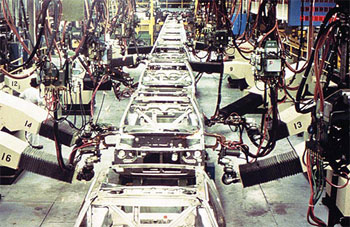
\includegraphics[scale=0.6]{img/unimate.jpg}
  		\caption{Unimate, General Motors}
  		\label{fig:unimate}
   	\end{minipage}\hfill
   	\begin {minipage}{0.48\textwidth}
     	\centering
     	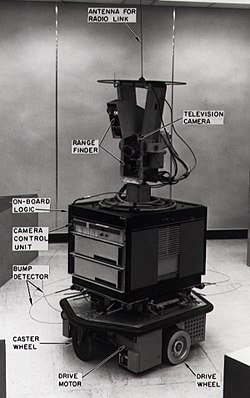
\includegraphics[scale=0.6]{img/shakey.jpg}
     	\caption{shakey en 1972}
     	\label{fig:shakey}
	\end{minipage}
\end{figure}

En 1970 se continua con la dinámica de crecimiento del sector, debido esta vez a la evolución del software ocurrida en esta época, y no parará hasta nuestros días, teniendo un crecimiento exponencial con una fuerte correlación con la evolución de software y hardware en general.
Desde este momento todas las grandes empresas dotaran sus fábricas de robots industriales. 

No es hasta 1996 cuando la empresa japonesa Honda presentó el robot P2, robot bípedo con forma humana que era capaz de caminar, empujar objetos, subir o bajar escaleras.
En la actualidad uno de los mayores logros en el mundo de la robótica se da en 2011, la NASA lanzó al espacio el robot tipo vehículo explorador \textit{Curiosity} \ref{fig:curiosity} , que aterrizó en Marte al año siguiente. Su principal cometido es investigar la capacidad pasada y presente del planeta para alojar vida.

\begin{figure}[H]
    \centering
    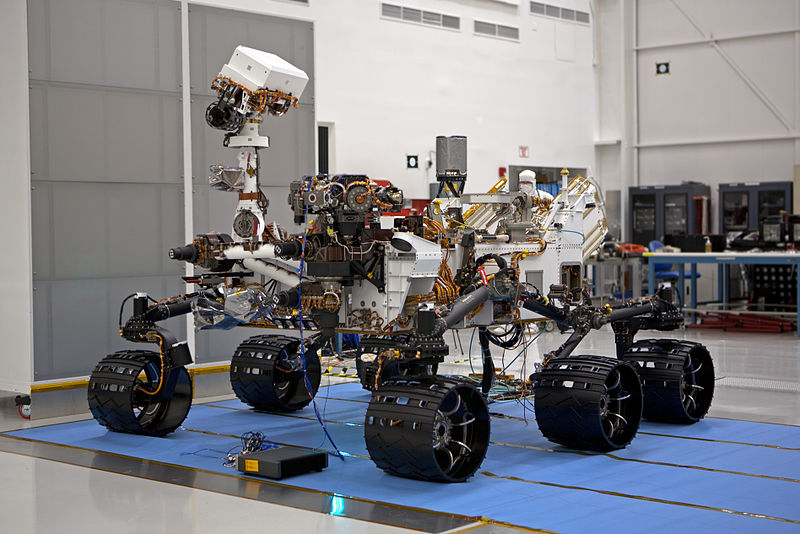
\includegraphics[scale=0.95]{img/curiosity.jpg}
  	\caption{El Curiosity en el Laboratorio de Propulsión a Chorro de la NASA}
  	\label{fig:curiosity}
\end{figure}

\subsection{Diferentes aplicaciones}
\label{subsec:diferentes aplicaciones}

Actualmente la robótica se encuentra en muchos ambitos de nuestra vida cotidiana, algunas aplicaciones son:
\begin{itemize}
\item \textbf{Robótica educativa}: Es una disciplina que trabaja en la concepción creación e implementación de prototipos robóticos y programas con fines pedagógicos. Con ello se permite al alumno fabricar sus representaciones sobre los fenómenos del mundo, facilitar su adquisición y trasferencia a distintas áreas de conocimiento.
A través de la robótica educativa, los docentes pueden desarrollar de una forma práctica los conceptos teóricos que suelen ser abstractos y confusos, además despierta el interés del alumno por esos temas y relaciona al niño con el mundo tecnológico en el que se mueve. El empleo de un ambiente de aprendizaje basado en la robótica educativa ayuda al desarrollo de nuevas habilidades y conceptos, fortalece el pensamiento lógico, estructurado y formal del alumnado, desarrollando su capacidad para resolver problemas concretos.
Una de las características de este ámbito es la capacidad que posee para mantener la
atención del alumno, ya que manipula y experimenta haciendo que se concentre en sus
percepciones y observaciones sobre la actividad que realiza. Actualmente existen varios kits de robótica, algunos de ellos son: LEGO MINDSTORMS education, LEGO WeDo, LEGO NXT o Parallax Scribbler. Además, también existe la posibilidad de trabajar con programas con los que controlar y simular diferentes La robótica en Educación Infantil. Realidades y limitaciones robots como son NXT-G Educación, ROBOTC, ROBOLAB o Microsoft Robotics Developer Studio.

\item \textbf{Medicina}: involucra en si varios ámbitos ya sea en cirugías de alto riesgo, en rehabilitaciones, en ayuda a personas con enfermedades de movilidad o discapacitados, en el almacenamiento de medicamentos y también en lo que se trata en pruebas ficticias y cirugías computarizadas.

\item \textbf{Militar}: la robótica donde más ha evolucionado es en la creación de vehiculos autónomos, tecnología que tras unos años pasa a a ser de uso civil.
Algunas de las creaciones que nos hemos heredados es el UAV, que se conocen comúnmente como dron, es una aeronave que vuela sin tripulación, Capaz de mantener de manera autónoma un nivel de vuelo controlado y sostenido, y propulsado por un motor de explosión, eléctrico, o de reacción.

\item \textbf{Robotica aeroespacial}: Uno de los mayores impulsores de la robótica ha sido la conquista del espacio, esta es una parte fundamental de la exploración espacial, debido a la imposibilidad de ser realizada en primera mano por un humano.
La idea básica sobre Robots Espaciales consiste en utilizar Inteligencia Artificial para
permitir a los robots realizar labores de exploración como si de un humano se tratase, desplazarse en terrenos y ambientes complejos de forma autónoma sin más conocimiento que lo recibido por sus sensores. Se busca no solo el proceso de pensamiento y análisis de los humanos en determinar las características del terreno, sino también la habilidad humana de conducir un vehículo en tiempo real.

\item \textbf{Industrial}
\item \textbf{Automovilismo}
\end{itemize}

\subsection{Tipos de Robots}
\label{subsec:tipos de robots}

Ningún autor se pone de acuerdo en cuántos y cuáles son los tipos de robots y sus características esenciales. La más común son la que a continuación se presentan:

\textbf{Segun su Estructura}:
\begin{itemize}
\item \textbf{Androides}: Un robot humanoide que se limita a imitar los actos y gestos de un controlador humano, no es visto por el público como un verdadero androide, sino como una simple marioneta animatrónica. El androide siempre ha sido representado como una entidad que imita al ser humano tanto en apariencia, como en capacidad mental e iniciativa

\item \textbf{Poliarticulados}: En este grupo pueden encontrarse robots de diversas formas y configuraciones, pero su característica en común es la de ser sedentarios. Es decir, que son robots estructurados para moverse en un determinado espacio de trabajo, según uno o más sistemas de coordenadas y con un número limitado de grados de libertad.

\item \textbf{Móviles}: estos robots cuentan con orugas, ruedas o patas que les permiten desplazarse de acuerdo a la programación a la que fueron sometidos. Estos robots cuentan con sistemas de sensores, que son los que captan la información que dichos robots elaboran. Los móviles son utilizados en instalaciones industriales, en la mayoría de los casos para transportar la mercadería en cadenas de producción así como también en almacenes. Además, son herramientas muy útiles para investigar zonas muy distantes o difíciles de acceder, es por eso que en se los utiliza para realizar exploraciones espaciales o submarinas.

\item \textbf{Zoomórficos}: la locomoción de estos robots imita a la de distintos animales y se los puede dividir en caminadores y no caminadores. Estos últimos están aún muy poco desarrollados mientras que los caminadores sí lo están y resultan útiles para la exploración volcánica y espacial.

\item \textbf{Híbridos}: Este término corresponde a todos aquellos robots que son difíciles de clasificar, ya que corresponden a una combinación de las estructuras anteriormente explicadas. Por ejemplo, un robot híbrido, que esté conformado por la segmentación de articulaciones y ruedas, podría ser considerado tanto móvil, así como zoomórfico.

\end{itemize}

\begin{figure}[H]
	\begin{minipage}{0.48\textwidth}
    	\centering
     	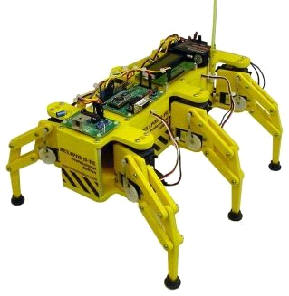
\includegraphics[scale=0.6]{img/robot-zoomorfico.jpg}
  		\caption{Robot zoomórfico}
  		\label{fig:unimate}
   	\end{minipage}\hfill
   	\begin {minipage}{0.48\textwidth}
     	\centering
     	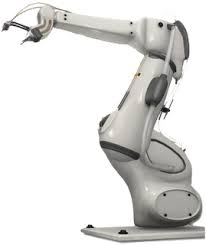
\includegraphics[scale=0.6]{img/robot-poliarticulado.jpg}
     	\caption{Robot poliarticulado}
     	\label{fig:shakey}
	\end{minipage}
\end{figure}


\textbf{Según su Cronología}:
\begin{itemize}
\item \textbf{1ª Generación. Manipuladores}: Son sistemas mecánicos multifuncionales con un sencillo sistema de control, bien manual, de secuencia fija o de secuencia variable.

\item \textbf{2ª Generación. Robots de aprendizaje}: Repiten una secuencia de movimientos de movimientos que ha sido ejecutada previamente por un operador humano. El modo de hacerlo es a través de un dispositivo mecánico. El operador realiza los movimientos requeridos mientras el robot le sigue y los memoriza.

\item \textbf{3ª Generación. Robots con control sensorizado}: El controlador es una computadora que ejecuta las órdenes de un programa y las envía al manipulador para que realice los movimientos necesarios.

\item \textbf{4ª Generación. Robots inteligentes}: Son similares a los anteriores, pero además poseen sensores que envían información a la computadora de control sobre el estado del proceso. Esto permite una toma inteligente de decisiones y el control del proceso en tiempo real.
\end{itemize}

\textbf{ROBOTICA EN MI TFG}


\section{Lenguajes de programación visual}
\label{sec:lenguajes}

Un lenguaje de programación visual es cualquier lenguaje de programación que permite a los usuarios crear programas manipulando elementos del programa gráficamente en lugar de especificarlos textualmente. Permite la programación con expresiones visuales, arreglos espaciales de texto y símbolos gráficos, utilizados como elementos de sintaxis o notación secundaria. Por ejemplo, muchos se basan en la idea de "cajas y flechas", donde las cajas u otros objetos de pantalla se tratan como entidades, conectadas por flechas, líneas o arcos que representan relaciones, mientras que otros se basan en el apilamiento de "cajas" con una funcion predefinida, creando así varios flujos de acciones programáticas con una objetivo final.

Estos lenaguajes por regla general se usan en programación dirigida por eventos, La programación dirigida por eventos es un paradigma de programación en el que el flujo del programa está determinado por eventos o mensajes desde otros programas o hilos de ejecución.
Las aplicaciones desarrolladas con programación dirigida por eventos implementan un bucle principal o main loop donde se ejecutan las dos secciones principales de la aplicación: El selector de eventos y el manejador de eventos.
HISTORIA

Podemos diferenciar varios niveles dentro de los lenguajes de programación visual:
\begin{itemize}
\item \textbf{Sintaxis}: en el nivel sintáctico, la explicación del bloque está limitada a
estructura del lenguaje. Por ejemplo, una explicación podría revelar que una condición es parte de una declaración \textit{IF} y no debe ser confundido con una acción que se puede ejecutar en \textit{THEN} o \textit{ELSE} parte de una declaración. Sin embargo, este no trata de definir de forma específica qué es lo que define esa condición.
Intentan reducir o incluso eliminar por completo los errores sintácticos y ayudan a la creación de programas bien formados. Una analogía sería el corrector ortográfico en procesadores de texto que subraya o incluso corrige automáticamente palabras o gramática individuales.	

\item \textbf{Semántica}: en el nivel de la semántica,se dan explicaciones sobre los bloques, a menudo implementadas a través de funciones de ayuda que describen el significado
de un bloque. El usuario obtiene una respuesta semántica en forma de panel de ayuda genérico incluyendo una breve descripción del significado del comando o bloque y la lista de opciones adicionales.

\item \textbf{Pragmática}: permiten llevar nuestra implementación a un punto de testeo específico, nos ayudan con una serie de módulos propios a crear el entorno necesario para simular el funcionamiento de nuestro programa en ese estado.
\end{itemize}

\subsection{Motivación}
\label{subsec:motivacion}
Las principales motivaciones del uso de estos lenguajes son su \textbf{accesibilidad}, ya que no requiere de una infraestructura potente para su funcionamiento.
Además el \textbf{facil aprendizaje} hace que sea un lenguaje idóneo para aquellos que no tienen ningún conocimiento de informática previo.
Y por último el eliminar de la ecuación algo tan simple como los \textbf{errores de sintaxis}, nos olvidamos completamente de este tipo de fallos, haciendo el desarrollo más fluido y menos frustrante para los principiantes, algo que puede marcar la diferencia a la hora de encontrar gratificante el desarrollo de aplicaciones con estos lenguajes.

\subsection{Tipos}
\label{subsec:tipos}

\begin{itemize}
\item \textbf{Blocly}: El desarrollo de Blockly comenzó en el verano de 2011, y el primer lanzamiento público fue en Maker Faire en mayo de 2012. Blockly fue originalmente diseñado como un reemplazo para OpenBlocks en App Inventor. [3] Neil Fraser comenzó el proyecto con Quynh Neutron, Ellen Spertus y Mark Friedman como colaboradores.
Es un proyecto de Google y es de código abierto bajo la licencia Apache 2.0  Por lo general, se ejecuta en un navegador web y se asemeja visualmente a Scratch. Blockly también se está implementando para Android e iOS aunque no todas las funciones basadas en el navegador web están disponibles para Android / iOS.
Utiliza bloques visuales que se unen entre sí para facilitar la escritura de códigos y generar código JavaScript, Python, PHP o Dart. También se puede personalizar para generar código en cualquier lenguaje de computadora textual.

\begin{figure}[H]
    \centering
    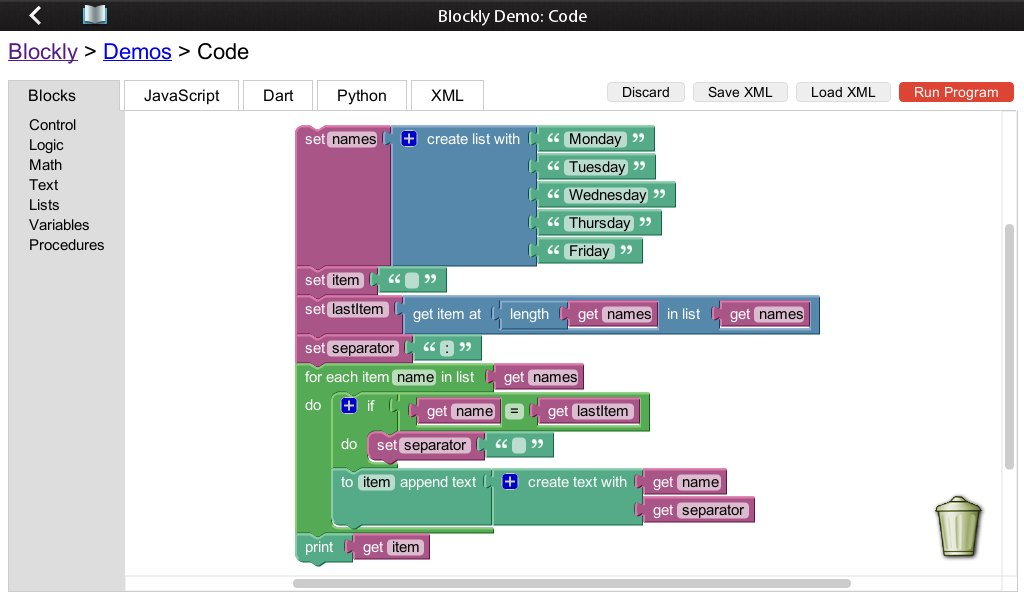
\includegraphics[scale=0.40]{img/blockly.jpg}
  	\caption{Lenguaje de programación visual Blockly}
  	\label{fig:blockly}
\end{figure}


\item \textbf{Scratch}:es un proyecto del Grupo Lifelong Kindergarten del MIT Media Lab.
Es utilizado por estudiantes y docentes de todo el mundo para expresar ideas mediante animaciones, juegos e interacciones facilmente programables con este entorno, hablaremos en capitulos siguientes.


\item \textbf{Snap!}:desarrollada por la Universidad de California en Berkeley, que sigue la filosofía de facilidad y sencillez para aprender a programar,  Snap se basa en el conocido programa de Scratch, siendo su uso más extendido entre edades más maduras que las de Scratch.
Snap está programado en JavaScript. Esto hace que podamos usarlo desde cualquier navegador, ya sea desde un ordenador como desde las tablets.
En las versiones actuales de Scratch (1.4 ó 2.0) se requiere el uso del plugin privativo de flash player. Si bien es cierto que a partir de la próxima versión 3.0 estará desarrollado íntegramente en HTML5 para que pueda funcionar en la mayoría de dispositivos móviles y tablets. Puedes acceder a este enlace para más información.

\begin{figure}[H]
    \centering
    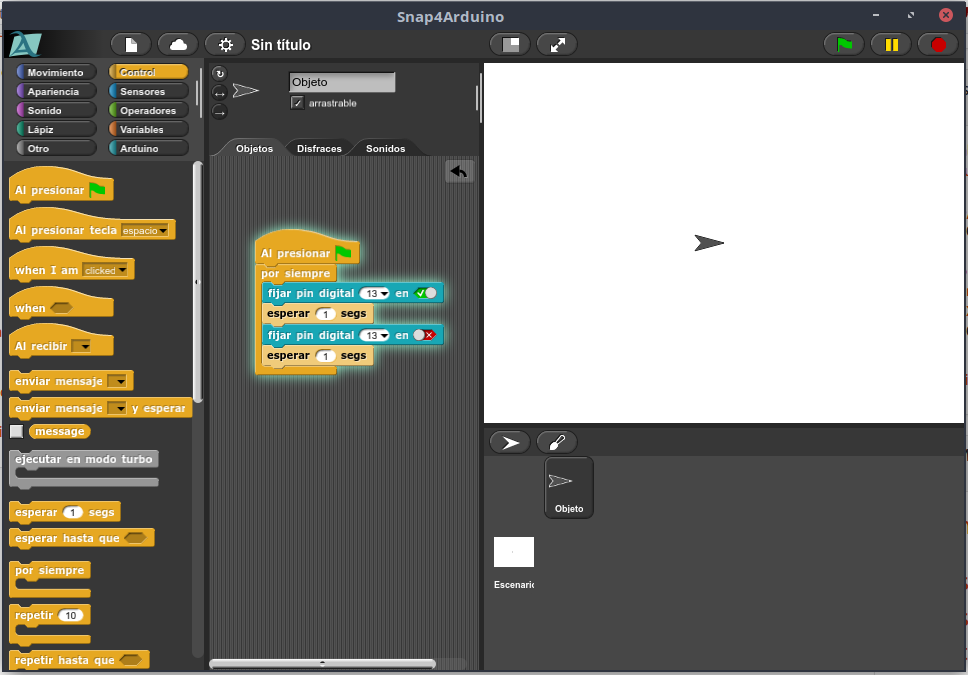
\includegraphics[scale=0.40]{img/snap.png}
  	\caption{Lenguaje de programación visual Snap!}
  	\label{fig:snap}
\end{figure}


\item \textbf{Kodu}: originalmente llamado Boku, es un entorno de desarrollo integrado de programación (IDE) de los laboratorios FUSE de Microsoft. Se ejecuta en Xbox 360 y Microsoft Windows XP, Windows Vista, Windows 7, Windows 8 y Windows 10. Fue lanzado en el Xbox Live Marketplace el 30 de junio de 2009. Una versión de Windows está disponible para el público en general para su descarga desde el portal web FUSE de Microsoft. 

\end{itemize}